\documentclass[10pt,aspectratio=169]{beamer}

\usetheme{Madrid}
\usecolortheme{seahorse}
\useinnertheme{rectangles}
\useoutertheme{miniframes}

\usepackage[utf8]{inputenc}
\usepackage{graphicx}
\graphicspath{{ADEPT/data/models/rf/}}
\usepackage{booktabs}
\usepackage{xcolor}
\usepackage{tikz}
\usepackage{array}
\usepackage{colortbl}

\definecolor{good}{RGB}{34,139,34}
\definecolor{warn}{RGB}{200,140,0}
\definecolor{bad}{RGB}{180,40,40}

\newcommand{\good}[1]{\textcolor{good}{\textbf{#1}}}
\newcommand{\warn}[1]{\textcolor{warn}{\textbf{#1}}}
\newcommand{\bad}[1]{\textcolor{bad}{\textbf{#1}}}

\title[ADEPT --- RF Results]{ADEPT --- Random Forest Base Learner}
\subtitle{Phase 2 Results: Analysis and Next Steps}
\author{Guilherme Leit\~ao}
\institute[IST/INESC-ID]{Master Thesis --- IST / INESC-ID}
\date{\today}

\begin{document}

% ============================================================
\begin{frame}
  \titlepage
\end{frame}

% ============================================================
\begin{frame}{What was trained}
\begin{itemize}
  \item \textbf{Task:} binary classification on the 24-dim per-window aggregates from Phase~1
  (\texttt{rf\_stats.npy}). Positive class = TANTGen-perturbed window;
  negative class = 4 matched benign sources (ddos, dos\_slow, mirai, ssdp\_flood) ---
  the only attacks for which TANTGen produced structurally valid adversarial PCAPs
  (portscan / syn\_dos excluded: 1--2 packet flows; fuzzing excluded: snaplen no-op).
  \item \textbf{Test split:} flow-atomic, stratified by source ($\sim$369k windows;
  59\% adversarial / 41\% benign --- 3 modes per attack make adversarial-majority).
  \item \textbf{Best hyperparameters} (grid search, val macro-F1):
  \texttt{n\_estimators=200}, \texttt{max\_depth=None}, \texttt{min\_samples\_leaf=1}.
\end{itemize}

\begin{block}{Headline metrics (test, overall)}
\centering
\begin{tabular}{lcccc}
\toprule
\textbf{Macro F1} & \textbf{ROC AUC} & \textbf{PR AUC} & \textbf{Recall (adv)} & \textbf{Precision (adv)} \\
\midrule
\good{0.987} & \good{0.997} & \good{0.996} & 0.994 & 0.985 \\
\bottomrule
\end{tabular}
\end{block}
\end{frame}

% ============================================================
\begin{frame}{Confusion matrix \& curves}
\begin{columns}[t]
\column{0.33\linewidth}
\centering
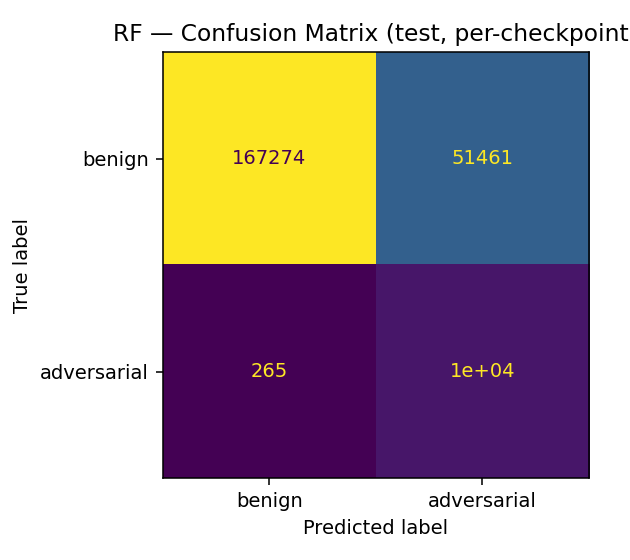
\includegraphics[width=\linewidth]{confusion_matrix.png}\\[2pt]
{\scriptsize Confusion Matrix}

\column{0.33\linewidth}
\centering
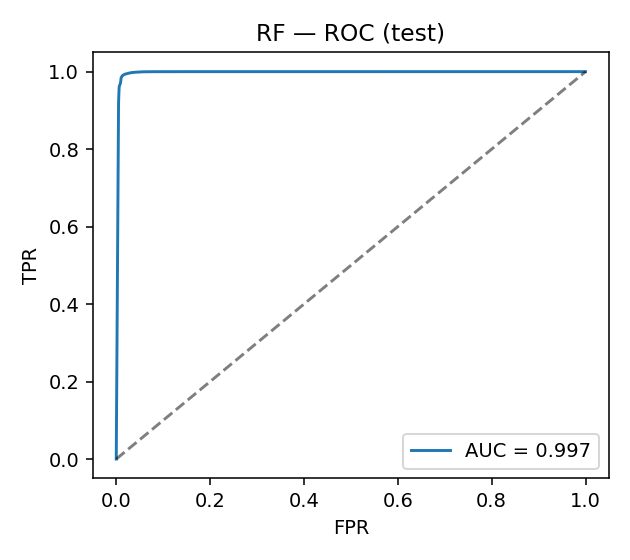
\includegraphics[width=\linewidth]{roc_curve.png}\\[2pt]
{\scriptsize ROC (AUC = 0.997)}

\column{0.33\linewidth}
\centering
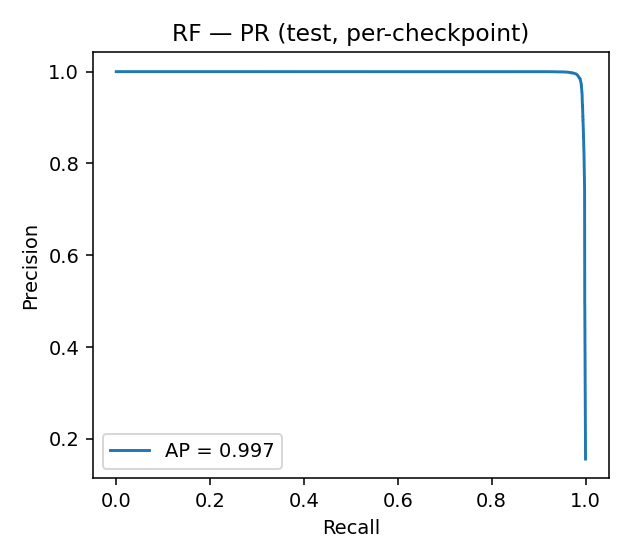
\includegraphics[width=\linewidth]{pr_curve.png}\\[2pt]
{\scriptsize Precision--Recall (AP = 0.996)}
\end{columns}

\vspace{0.5em}
\begin{itemize}\small
  \item Strong global separability between benign and TANTGen-adversarial windows.
  \item PR curve nearly overlapping ROC confirms the 59/41 adversarial-majority imbalance is
        well handled by the \texttt{class\_weight=balanced\_subsample} setting.
\end{itemize}
\end{frame}

% ============================================================
\begin{frame}{Per-variant performance (vs. balanced benign)}
\centering\small
\begin{tabular}{lccc}
\toprule
\textbf{Variant} & \textbf{F1$_\text{adv}$} & \textbf{ROC AUC} & \textbf{PR AUC} \\
\midrule
\rowcolor{good!15} ddos\_adv\_\{both, iat, size\}        & 0.91 / 0.90 / 0.91 & 0.995--0.998 & 0.917--0.957 \\
\rowcolor{good!15} dos\_slow\_adv\_\{both, iat, size\}   & 0.955 / 0.953 / 0.955 & 0.997--0.998 & 0.977--0.980 \\
\rowcolor{good!15} ssdp\_flood\_adv\_\{both, iat, size\} & 0.91 / 0.91 / 0.91 & 0.998        & 0.959 \\
\rowcolor{warn!15} mirai\_adv\_both / iat                & 0.887 / 0.883      & 0.994--0.995 & 0.653--0.708 \\
\rowcolor{warn!15} mirai\_adv\_size                      & \warn{0.761}       & 0.983        & \warn{0.433} \\
\bottomrule
\end{tabular}

\vspace{0.6em}
\begin{itemize}\small
  \item \good{DDoS / DoS Slow / SSDP Flood:} strong detection across all three perturbation
        modes --- these are the variants ADEPT must catch.
  \item \warn{Mirai:} acceptable on \texttt{both}/\texttt{iat}; \warn{size-only noticeably weaker}
        (small payload-padding signal; low PR AUC reveals class-boundary fragility).
\end{itemize}
\end{frame}

% ============================================================
\begin{frame}{Same-base vs.\ balanced benign: where detection is harder}
Each variant is scored against two benign pools.
\textbf{Balanced:} K\,$\times$\,n\_adv windows drawn from all test benign (slide 4).
\textbf{Same-base:} only benign windows from the \emph{same} source capture.

\centering\small
\begin{tabular}{lcc>{\columncolor{warn!10}}c}
\toprule
\textbf{Variant} & \textbf{F1 (balanced)} & \textbf{F1 (same-base)} & \textbf{$\Delta$} \\
\midrule
\rowcolor{good!15} ddos\_adv\_\{both, iat, size\}        & 0.91 / 0.90 / 0.91 & 1.00 / 0.99 / 1.00 & $+$0.09 \\
\rowcolor{good!15} dos\_slow\_adv\_\{both, iat, size\}   & 0.955 / 0.953 / 0.955 & 1.00 / 1.00 / 1.00 & $+$0.05 \\
\rowcolor{good!15} ssdp\_flood\_adv\_\{both, iat, size\} & 0.91 / 0.91 / 0.91 & 0.99 / 0.99 / 0.99 & $+$0.08 \\
\rowcolor{warn!15} mirai\_adv\_both / iat                & 0.887 / 0.883 & 0.667 / 0.660 & \warn{$-$0.22} \\
\rowcolor{warn!15} mirai\_adv\_size                      & 0.761         & \warn{0.553}  & \warn{$-$0.21} \\
\bottomrule
\end{tabular}

\vspace{0.5em}
\begin{itemize}\small
  \item \good{Volumetric attacks:} same-base F1 \emph{exceeds} balanced F1 ---
        TANTGen's IPAT shifts are so pronounced that detection is easy even
        against same-source benign traffic.
  \item \warn{Mirai:} same-base F1 drops by $\sim$0.21--0.22 ---
        \emph{capture-specific bleed}: same-flow benign and adversarial Mirai
        windows share underlying timing patterns, making them harder to separate
        when the benign pool is restricted to the same capture.
\end{itemize}
\end{frame}

% ============================================================
\begin{frame}{Feature importance}
\begin{columns}[T]
\column{0.52\linewidth}
\centering
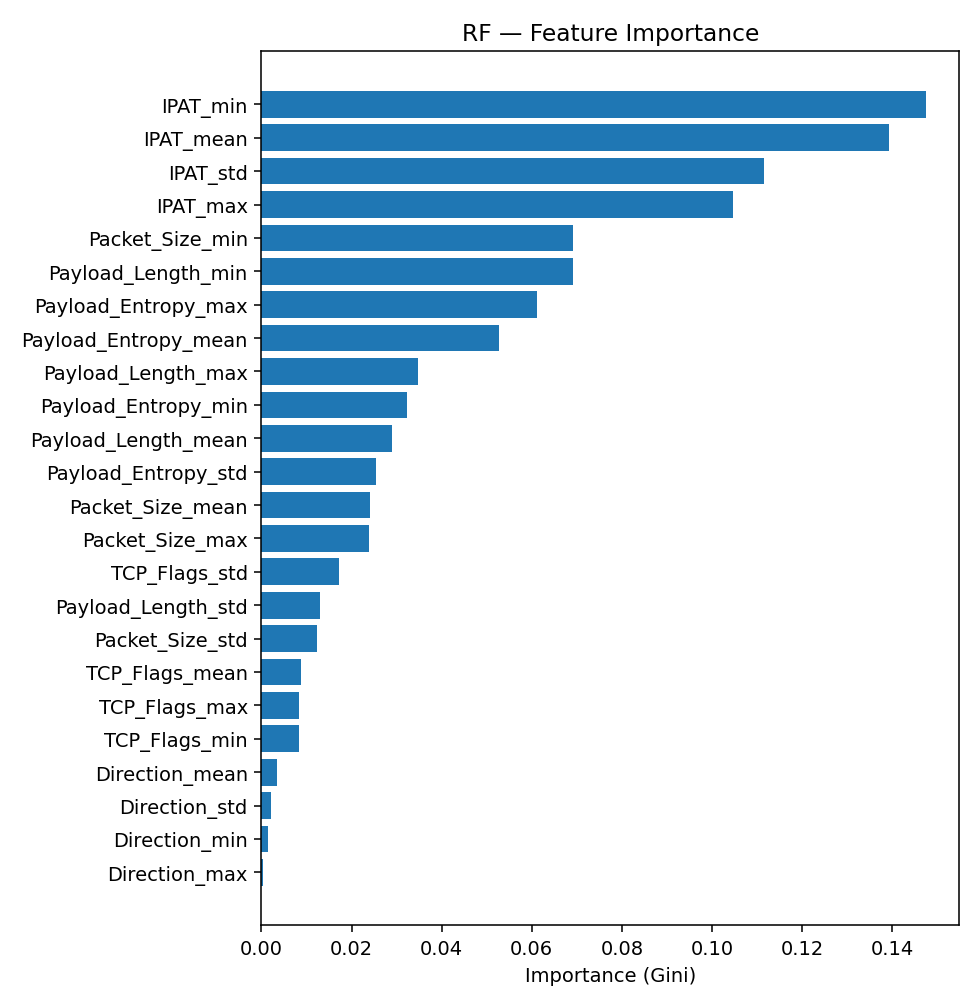
\includegraphics[width=\linewidth,height=0.72\textheight,keepaspectratio]{feature_importance.png}

\column{0.48\linewidth}
\textbf{Top discriminators}
\begin{itemize}\scriptsize
  \item IPAT statistics (mean / std / min / max) dominate --- TANTGen's
        timing perturbations are the strongest signal.
  \item Packet\_Size and Payload\_Length aggregates contribute
        meaningfully on the \texttt{size}/\texttt{both} modes.
  \item Direction and TCP\_Flags aggregates --- secondary, mostly useful
        for capture identification rather than perturbation detection.
\end{itemize}

\vspace{0.4em}
\textbf{Implication:}\\\scriptsize
Before training, each of the 24 features is standardized using a mean and
standard deviation computed \emph{jointly} from both benign and adversarial
windows (\texttt{mean\_std.json}). This means the RF sees every feature as
a z-score --- how far a window deviates from the combined population average.
Because TANTGen's timing perturbations shift inter-packet arrival times well
outside the joint mean, those IPAT z-scores become the dominant discriminative
signal for the model.
\end{columns}
\end{frame}

% ============================================================
\begin{frame}{Conclusions}
\begin{enumerate}
  \item \good{On the principled 4-attack dataset (ddos, dos\_slow, mirai,
        ssdp\_flood), the 24-dim RF reaches 0.987 macro-F1 / 0.996 PR-AUC}
        --- a strong baseline for the statistical half of the ADEPT ensemble.
  \item \good{Volumetric attacks (DDoS, DoS Slow, SSDP Flood) are
        strongly detected across all three perturbation modes} ---
        same-base F1 $\geq$ 0.99, confirming IPAT shifts are the dominant signal.
  \item \warn{The size-only mode is consistently weakest --- expected,
        since RF aggregates compress per-packet padding into mean/std/min/max.
        Mirai size drops furthest (F1 = 0.76, PR AUC = 0.43).}
  \item \warn{Mirai shows capture-specific bleed: same-base F1 drops
        0.21--0.22 below balanced F1 --- same-flow benign and adversarial
        windows share timing patterns the RF cannot fully untangle.}
  \item \bad{PortScan and SYN\_DoS are structurally incompatible with
        N-packet windowing} (1--2 packet flows yield $<$200 windows from
        $>$150k flows) --- excluded from training and evaluation.
  \item \bad{Fuzzing adversarials are snaplen-200B no-ops} ---
        excluded from training; their near-zero F1 confirms
        TANTGen produced no effective perturbation.
\end{enumerate}
\end{frame}

% ============================================================
\begin{frame}{Next steps}
\textbf{Short-term (End of May) --- complete the ensemble \& tune end-to-end}
\begin{enumerate}\scriptsize
  \item \textbf{Phase 3 --- TCN base learner} on \texttt{sequence.npy}.
        Dilated temporal convolutions should close the gap on \texttt{size}-only
        and Mirai variants where RF aggregates compress the signal.
  \item \textbf{Phase 4 --- Mini-Transformer meta-learner} fusing RF + TCN logits.
  \item \textbf{Sync with In\^es} on the TANTGen version in use --- confirm whether
        the Fuzzing snaplen-200B no-op is intrinsic or a fixable config issue.
  \item \textbf{DPSS hyperparameter sweep} --- script to grid-search the full pipeline:
        Packet-to-Tensor \texttt{window\_size} $\in \{5,10,20\}$ (smaller $N$ recovers
        PortScan / SYN\_DoS), extended RF grid, TCN \& Mini-Transformer params (TBD).
        Objective: maximize ensemble detection accuracy. Long-running --- hence offloaded.
\end{enumerate}

\textbf{Long-term --- defense layer \& write-up}
\begin{enumerate}\scriptsize\setcounter{enumi}{4}
  \item \textbf{Phase 5 --- Purification Transformer} (decoder-only Seq2Seq) projecting
        adversarial windows back onto the benign manifold; KV-caching for latency.
  \item \textbf{Phase 6 --- RL Adaptation Agent} re-weighting the ensemble online
        from TANTGen feedback + offline DPI validation.
  \item \textbf{Dissertation write-up.}
\end{enumerate}
\end{frame}

% ============================================================
\begin{frame}[fragile]{Reproducibility}
\textbf{Artifacts under} \texttt{ADEPT/data/models/rf/}
\begin{itemize}\small
  \item \texttt{rf.joblib} --- fitted classifier
        (\texttt{n\_estimators=200}, \texttt{max\_depth=None}, \texttt{min\_samples\_leaf=1})
  \item \texttt{metrics.json} --- overall + per-source (vs\_all / vs\_balanced /
        vs\_same\_base) + per-\texttt{label\_str}
  \item \texttt{split.npz}, \texttt{dataset.npz} --- exact train/val/test partition
  \item \texttt{training\_info.json} --- full grid-search trace
  \item \texttt{*.png} --- confusion matrix, ROC, PR, feature importance
\end{itemize}

\vspace{0.6em}
\textbf{Re-run from scratch}
\begin{block}{}
\small
\begin{verbatim}
python3 scripts/adversarial_generation/generate_adversarials.py
python3 scripts/packet_to_tensor/process_all_attacks.py --tantgen
python3 scripts/rf/run_rf.py
\end{verbatim}
\end{block}
\end{frame}

\end{document}
